\documentclass[11pt,a4paper,oneside,onecolumn]{article}

\usepackage[T1]{fontenc}
\usepackage[utf8]{inputenc}
\usepackage[english]{babel}

\usepackage[a4paper, top=2.5cm, bottom=2.5cm, left=2.5cm, right=2.5cm]{geometry}

% 1.5 line spacing
\usepackage{setspace}
\onehalfspacing
\usepackage{amsmath}
\usepackage{amssymb}
\usepackage{amsfonts}
\usepackage{bm}
\usepackage{mathtools}
\usepackage{graphicx}
\usepackage{float}
\usepackage{booktabs}
\usepackage{tabularx}
\usepackage{array}
\usepackage{subcaption}
\usepackage{datetime}
\usepackage{tikz}

\usepackage[numbers,sort&compress]{natbib}
\usepackage[hidelinks]{hyperref}
\usepackage{url}

\usepackage{titlesec}

\titleformat{\section}
  {\normalfont\large\bfseries}
  {\thesection}{1em}{}

\titleformat{\subsection}
  {\normalfont\normalsize\bfseries}
  {\thesubsection}{1em}{}

% Paragraph formatting
\setlength{\parindent}{1.5em}
\setlength{\parskip}{0pt}

\title{Aircraft Structure Scanning with Optimal Path Finding}
\author{Krzysztof Jamrozy}
\date{\today}

\begin{document}

\maketitle

\section*{Abstract}
The aim of this paper is to determine an optimal scanning path for a laser-equipped robotic platform inspecting an aircraft structure. The problem description focuses on the differences between analytical and numerical approximations. More specifically, the goal is to avoid complicated calculations and transformations by using a PPO model to learn a control policy for the rover or a fleet of rovers.

\section{Introduction}
Scanning a structure requires time and repeated movements of an actuator. The obvious idea is to automate this task using a sophisticated system. Such a system could consist of a robotic platform or even an entire fleet of robots scanning the structure of an object. In this paper, there are two main approaches to determining how the robotic system should perform scanning in order to achieve an optimal, repeatable solution. One possible approach is to use geometric decomposition to simplify complex geometric shapes into simpler ones \cite{chandrajit1994geometry}, calculate optimal solutions for each generated shape (dynamic programming), and combine these solutions into a general solution for the given complex shape. The other possible approach is to use Machine Learning to train the system to handle a given geometry.


\section{Problem Description}
The given problem is to scan the surface of an aircraft to detect cracks or deformations. The task is relatively easy for a human: simply scan the surface and check the monitor for any suspicious areas. For a robotic system, the requirement is to acquire the data and identify the correct shape to avoid scanning other objects. The system needs to be flexible enough that it does not require a huge database of aircraft, but instead uses a smart algorithm to perform the task during execution. In other words, it needs to follow a set of rules that will complete the scanning process regardless of different sizes, surface complexities, or geometric features. 

\begin{figure}[htbp]
\centering
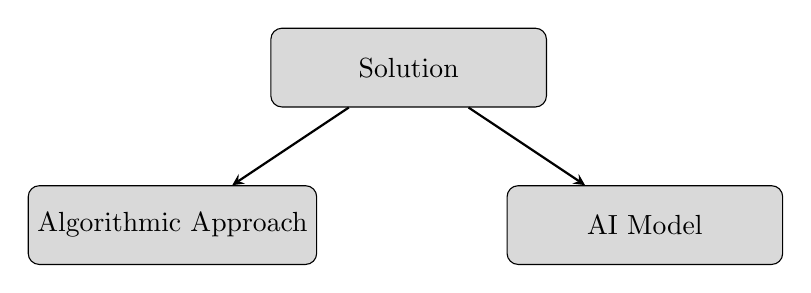
\begin{tikzpicture}[
    block/.style={
        rectangle,
        rounded corners,
        minimum width=3.5cm,
        minimum height=1cm,
        text centered,
        draw=black,
        fill=gray!30
    },
    arrow/.style={thick, ->, >=stealth}
]

\node[block] (sol) at (0,2) {Solution};
\node[block] (alg) at (-3,0) {Algorithmic Approach};
\node[block] (ai) at (3,0) {AI Model};

\draw[arrow] (sol) -- (alg);
\draw[arrow] (sol) -- (ai);

\end{tikzpicture}
\caption{Possible approaches to solving the problem}
\label{fig:approaches}
\end{figure}

While communication architecture is designed on simple TCP server-client model:

\begin{figure}[htbp]
\centering
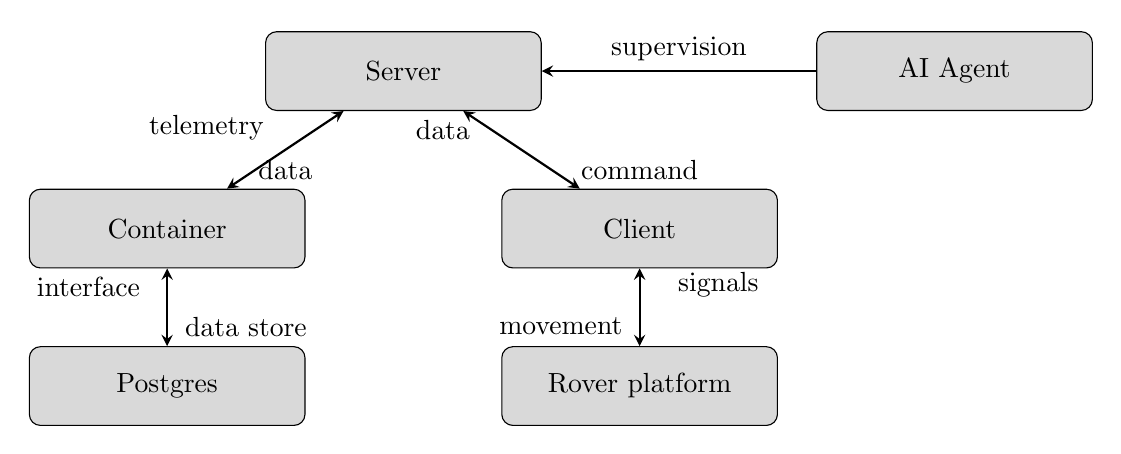
\begin{tikzpicture}[
    block/.style={
        rectangle,
        rounded corners,
        minimum width=3.5cm,
        minimum height=1cm,
        text centered,
        draw=black,
        fill=gray!30
    },
    arrow/.style={thick, ->, >=stealth},
    arrow2/.style={thick, <->, >=stealth}
]

  \node[block] (agent) at (7,2) {AI Agent};
  \node[block] (server) at (0,2) {Server};

  \node[block] (con) at (-3,0) {Container};
  \node[block] (post) at (-3,-2) {Postgres};

  \node[block] (client) at (3,0) {Client};
  \node[block] (rover) at (3,-2) {Rover platform};

  \draw[arrow] (agent) -- node[above] {supervision} (server);
  \draw[arrow2] (server) -- node[below] {data} node[above, xshift = -10mm] {telemetry} (con);
  \draw[arrow2] (server) -- node[above, xshift = -10mm] {data} node[below, xshift = 15mm] {command} (client);

  \draw[arrow2] (client) -- node[below, xshift = -10mm] {movement} node[above, xshift=10mm] {signals} (rover);
  \draw[arrow2] (con) -- node[above, xshift = -10mm] {interface} node[below, xshift = 10mm] {data store} (post);

\end{tikzpicture}
\caption{Proposed communication architecture}
\label{fig:comunication}
\end{figure}


\section{Classical Geometry with Dynamic Programming}

Decomposition is the process of dividing a complex object into simpler components or removing additional features to obtain simpler elements. The idea is to simplify complex shapes of aircraft structures into shapes that are easier to analyze. This approach requires some practice, but once mastered, it allows us to approximate or even fully calculate complex geometries.

One of the solutions for coverage path planning is convex decomposition \cite{mdpi2019convex}. The idea is to decompose an area into convex sub-areas \cite{mdpi2019convex}. Path planning in this scenario provides a sufficient coverage path so that the gaps between paths are kept to the minimum required.

For more curved shapes, it is feasible to draw a grid over the shape and treat it as a polygon (the denser the grid, the higher the coverage resolution and the smaller the overestimation). Convex decomposition requires some initial threshold for the minimum area division to prevent excessively high resolution or the creation of paths from infinitely small areas.

Another solution is Morse cellular decomposition. This method uses the critical points of a given function, such that

\[ dh_p = \left[ \frac{\partial h}{\partial x_1}(p) \quad \ldots \quad \frac{\partial h}{\partial x_N}(p) \right] \]

where

\[ \frac{\partial h}{\partial x_1}(p) = \ldots = \frac{\partial h}{\partial x_N}(p)= 0,\]

A critical point is non-degenerate if the Hessian matrix is nonsingular \cite{carriege2002morse}: 

\begin{equation}
H_h(p) =
\begin{bmatrix}
\frac{\partial^2 h}{\partial x_1^2}
& \cdots &
\frac{\partial^2 h}{\partial x_1 \partial x_N} \\
\vdots & \ddots & \vdots \\
\frac{\partial^2 h}{\partial x_N \partial x_1}
& \cdots &
\frac{\partial^2 h}{\partial x_N^2}
\end{bmatrix}_{p},
\qquad
\det(H_h(p)) \neq 0.
\end{equation}

By combining these decomposition methods, we can estimate the length (and time) of the complete path required to cover the shape or shapes.

\section{PPO-based Path Planning}
AI models are widely used in optimal path planning \cite{kufa2025pathplanning}. Most of the work is focused on obstacle avoidance or exploration management. Machine Learning in robotics requires flexibility to adjust robot behavior during operation. Reinforcement Learning offers significant advantages in robot control, but training a machine outside simulation could be dangerous. One promising approach is Proximal Policy Optimization (PPO) introduced by OpenAI \cite{schulman2017ppo}. The  idea is to use 2 components: the Actor and the Critic. The first one is responsible for generating/adjusting policies and the second one for estimating expected future returns. The advantage estimate indicates whether a selected action is better or worse than expected. Changes in action probabilities are represented by the policy probability ratio:

\begin{equation}
r_t(\theta) = \frac{\pi_{\theta}(a_t \mid s_t)}{\pi_{\theta_{\mathrm{old}}}(a_t \mid s_t)}
\end{equation}

The clipping mechanism in the surrogate objective function limits the benefit of excessively large policy updates, encouraging more stable training. Hyperparameter $\epsilon$ defines the clipping interval around the probability ratio of 1:

\begin{equation}
  L^{CLIP} (\theta) = \mathbb{E} [\min(r_t(\theta)\hat{A_t}, \operatorname{clip}(r_t(\theta), 1-\epsilon, 1+\epsilon)\hat{A_t})]
\end{equation}

Therefore an important aspect of this approach is that the model learns through trial and error similarly to human with no prior experience of the task. It is easy to judge if the model is making an obvious mistake or achieves sufficient path coverage. It is also possible to apply a trained model to a similar task without restarting the training process from scratch. This may be more difficult with classical geometric methods in analytical decomposition.

\section{AI Approach Testing}
Applying Reinforcement Learning to this problem requires a training environment. To present the test results, a functional simulation environment was created (Figure \ref{simulation_fig}). The robot, represented by a red point, is equipped with a laser beam, shown as a green circle, that scans the surrounding area. The environment distinguishes empty space (white) from the target object (gray). The side panel allows the user to adjust simulation parameters and initial conditions. The controls below the plots are used to manage training and simulation.

The initial experiment considers a simple circular region with the rover positioned inside the target area. The environment is defined as a 150 × 150 computational plane, with a laser beam diameter of 5 simulation units, a turning angle of 5°, and a required surface coverage of 98\%. The rover starts at (50, 50). The objective is to generate a scanning trajectory that satisfies the coverage requirement. The model is evaluated after 250, 500, and 1000 training episodes. The following figures compare the agent's behavior during training.

\begin{figure}[H]
  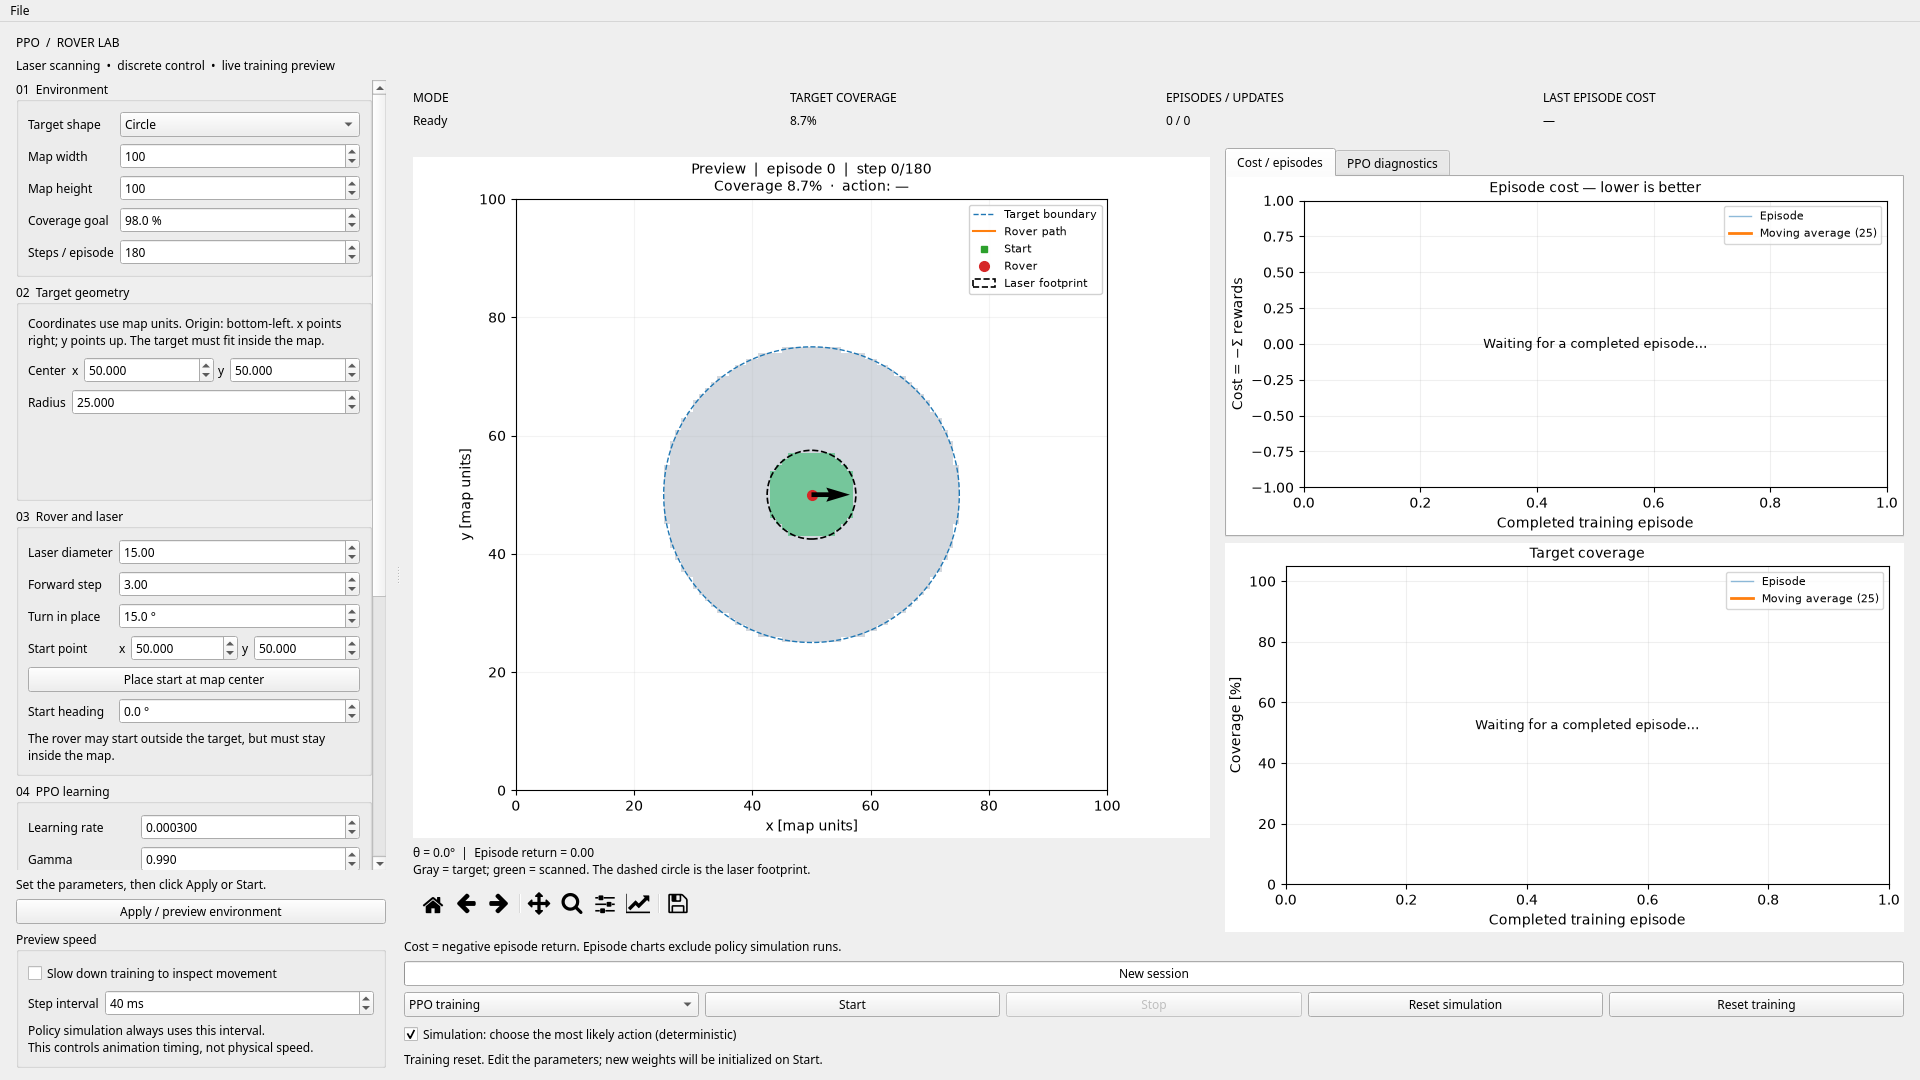
\includegraphics[width=\textwidth, keepaspectratio]{./images/simulation.png}
  \caption{Simulation environment\label{simulation_fig}}
\end{figure}

\begin{figure}[H]
  \centering
  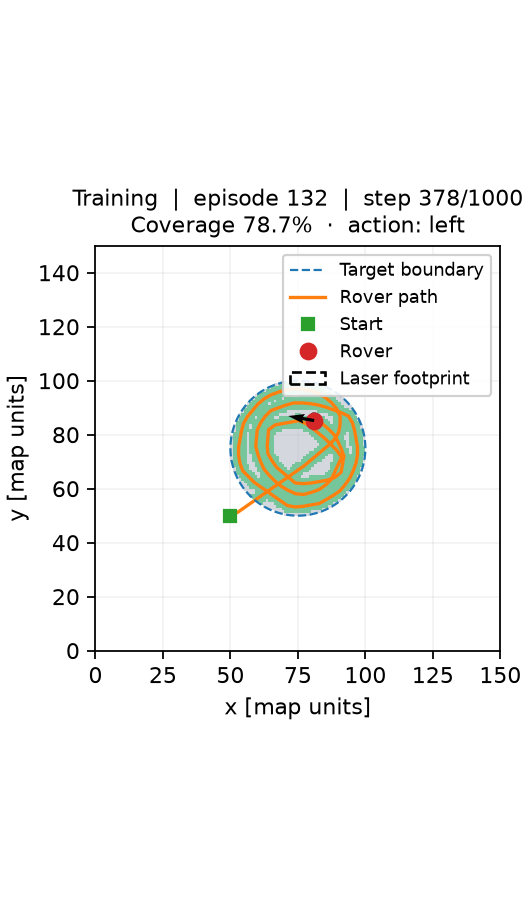
\includegraphics[width=0.3\textwidth, keepaspectratio]{./images/circle_250episodes/rover.png}
  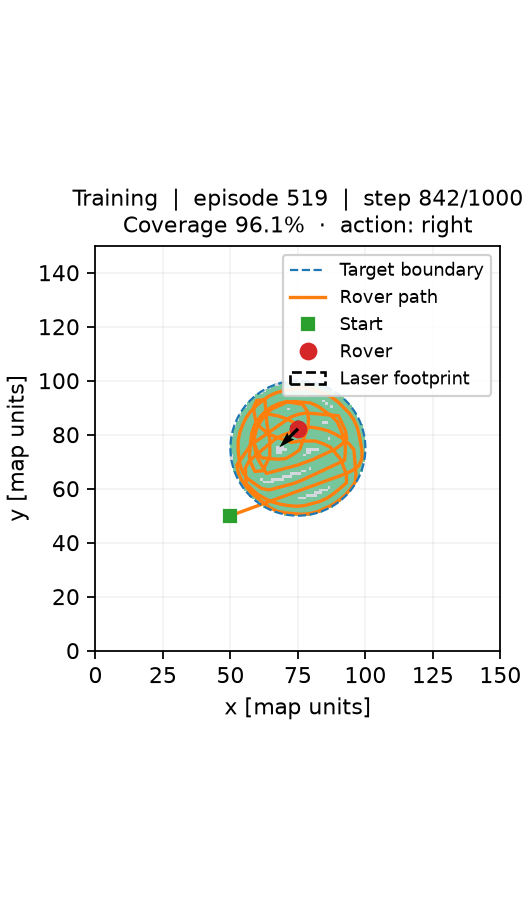
\includegraphics[width=0.3\textwidth, keepaspectratio]{./images/circle_500episodes/rover.png}
  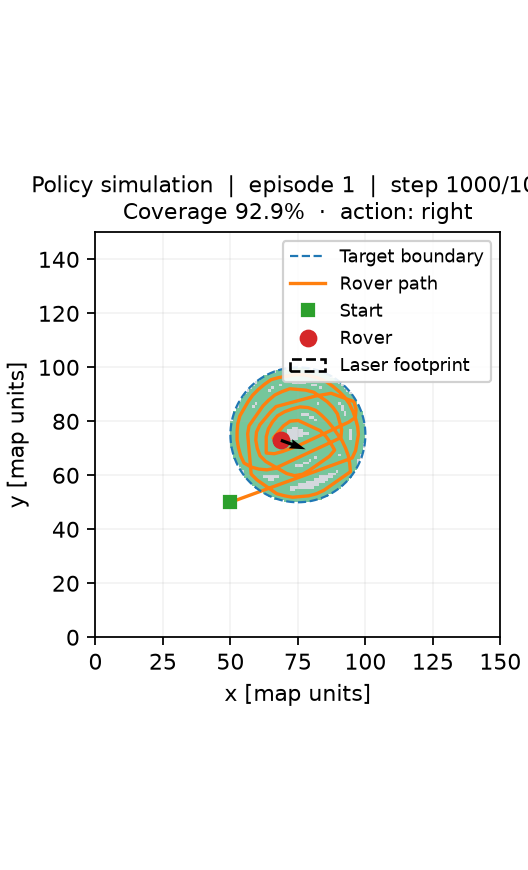
\includegraphics[width=0.3\textwidth, keepaspectratio]{./images/circle_1000episodes/rover.png}
  \caption{Comparison of scanning trajectories after 250, 500 and 1000 training episodes\label{training_output_fig}}
\end{figure}

\begin{figure}[H]
  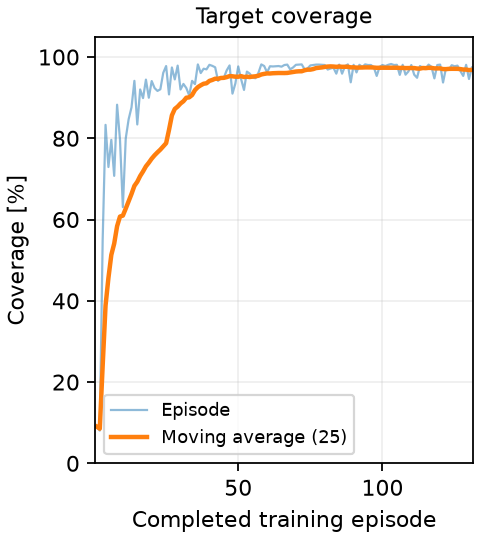
\includegraphics[width=0.3\textwidth, keepaspectratio]{./images/circle_250episodes/coverage.png}
  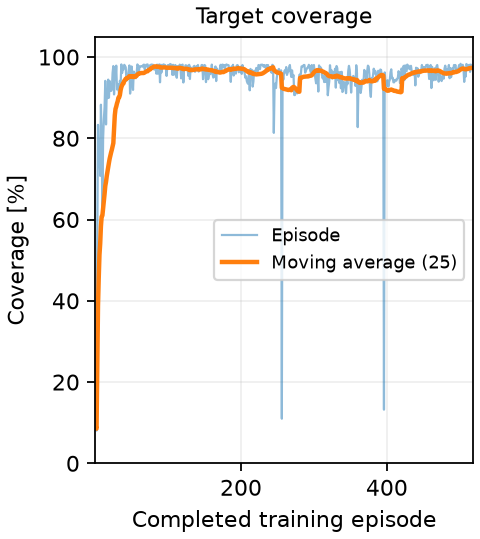
\includegraphics[width=0.3\textwidth, keepaspectratio]{./images/circle_500episodes/coverage.png}
  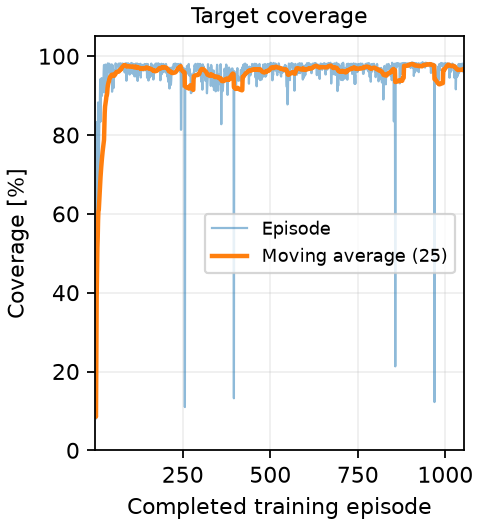
\includegraphics[width=0.3\textwidth, keepaspectratio]{./images/circle_1000episodes/coverage.png}
  \caption{Surface coverage comparison\label{cover_fig}}
\end{figure}

\begin{figure}[H]
  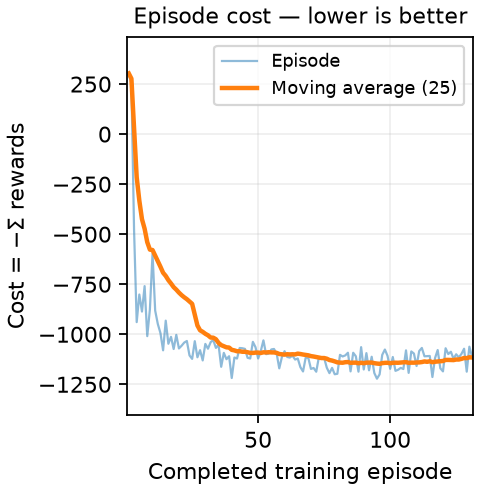
\includegraphics[width=0.3\textwidth, keepaspectratio]{./images/circle_250episodes/episode_cost.png}
  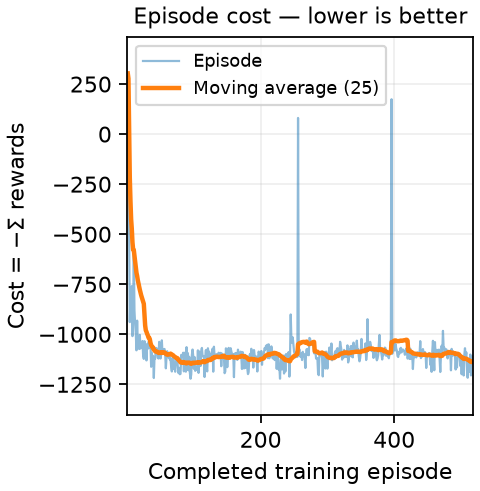
\includegraphics[width=0.3\textwidth, keepaspectratio]{./images/circle_500episodes/episode_cost.png}
  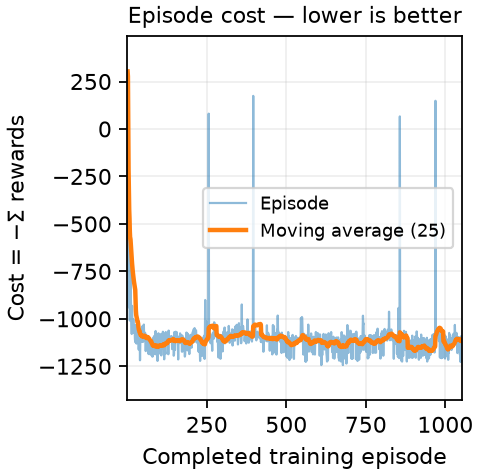
\includegraphics[width=0.3\textwidth, keepaspectratio]{./images/circle_1000episodes/episode_cost.png}
  \caption{Cost comparison \label{cost_fig}}
\end{figure}

\begin{figure}[H]
  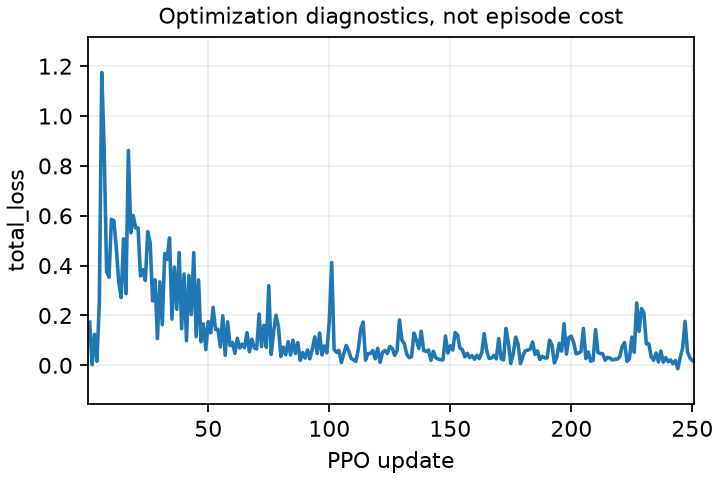
\includegraphics[width=0.29\textwidth, keepaspectratio]{./images/circle_250episodes/ppo_loss.png}
  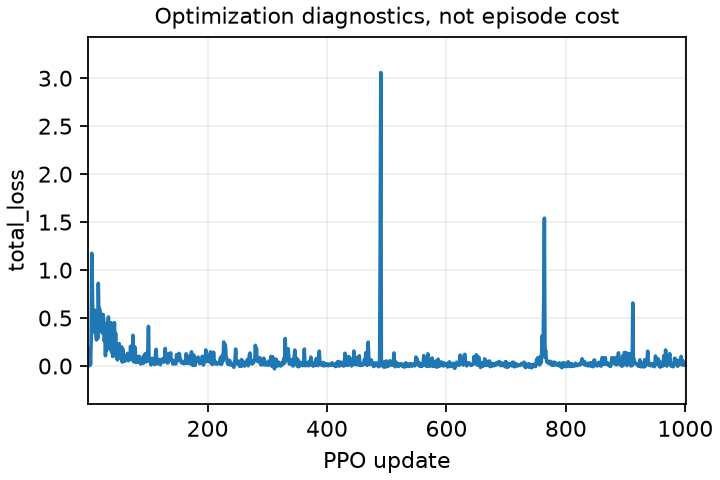
\includegraphics[width=0.29\textwidth, keepaspectratio]{./images/circle_500episodes/ppo_loss.png}
  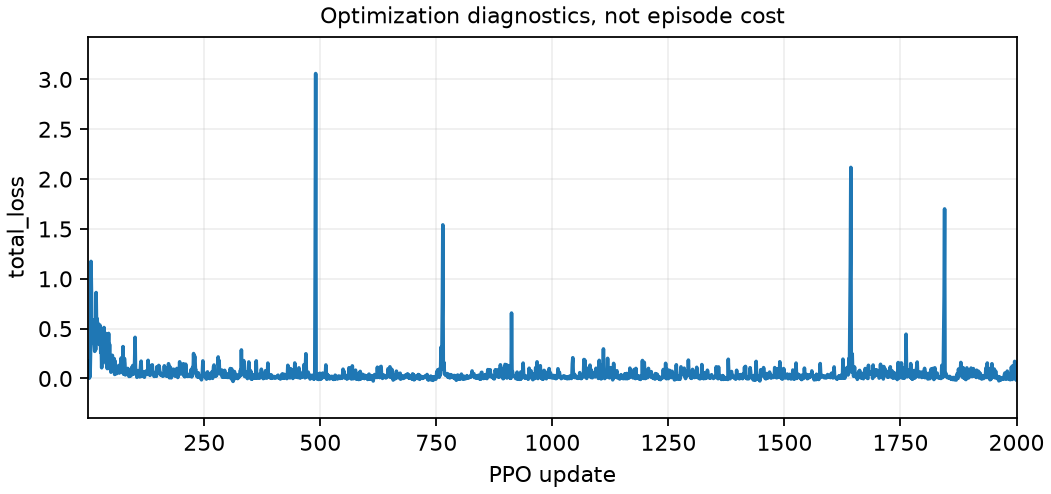
\includegraphics[width=0.42\textwidth, keepaspectratio]{./images/circle_1000episodes/ppo_loss.png}
  \caption{Loss function comparison \label{loss_function_fig}}
\end{figure}

An additional experiment was conducted using a triangular shape (point set in (40, 90), (100, 30) and (100, 90)) to approximate the geometry of an aircraft wing. As shown in Figure \ref{training_output_trian_fig}, a separately trained model can successfully handle a different geometric shape. Similar behavior was observed for an elliptical region, minor radius equal to 30, major radius 60 and center point (70, 100), as shown on the figure \ref{training_output_ellipse_fig}. There the agent first had to locate the target area before beginning the scanning process.

These results provide preliminary evidence that specialized models could form the basis of a architecture build on simpler modules, potentially extending toward a Multi-Agent Reinforcement Learning (MARL) system.

\begin{figure}[H]
  \centering
  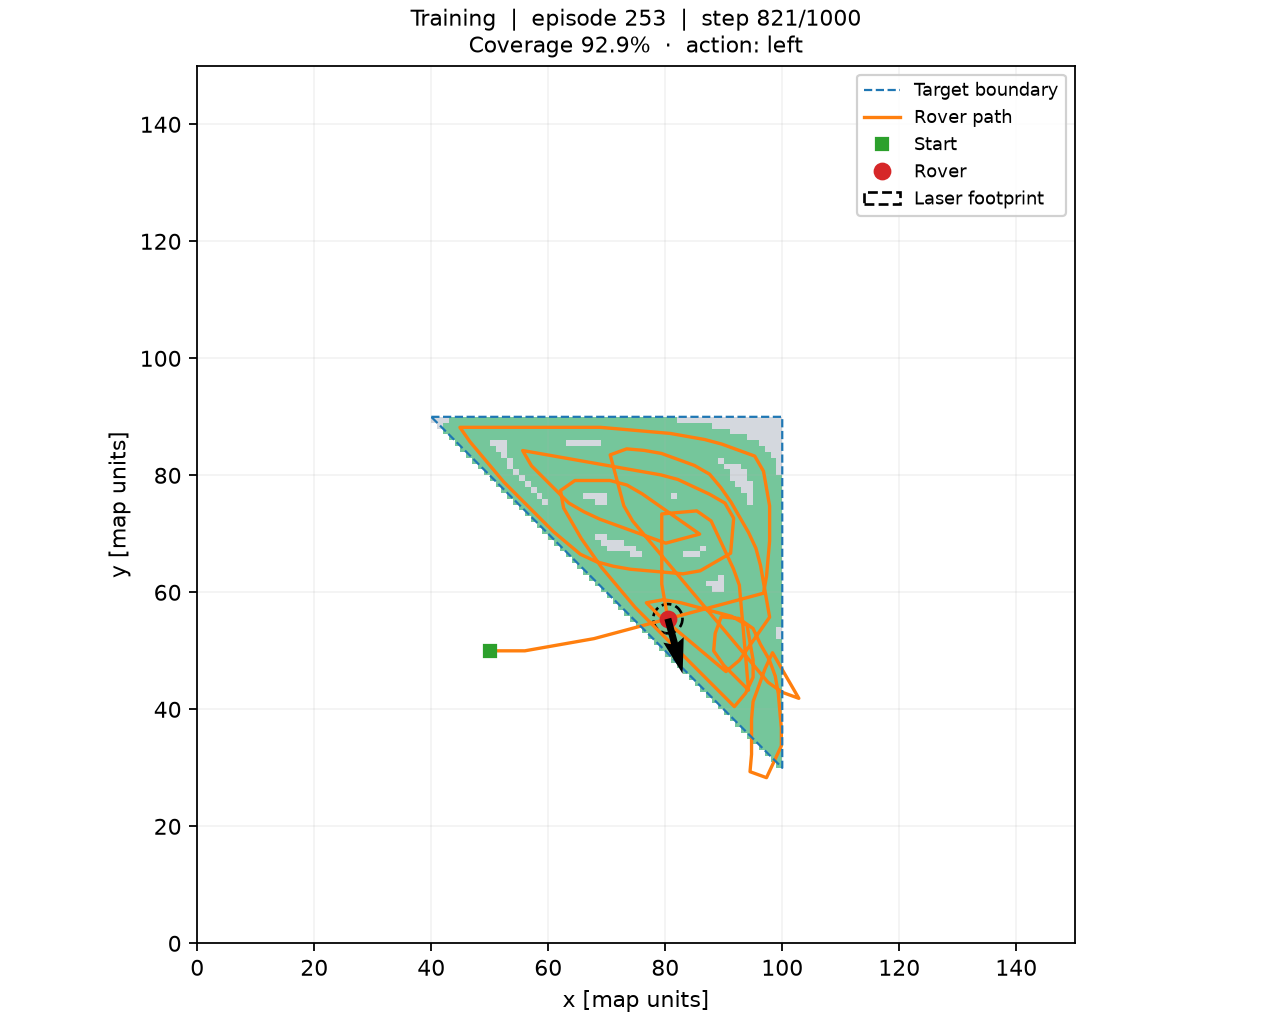
\includegraphics[width=0.3\textwidth, keepaspectratio]{./images/triangle_250episodes/rover.png}
  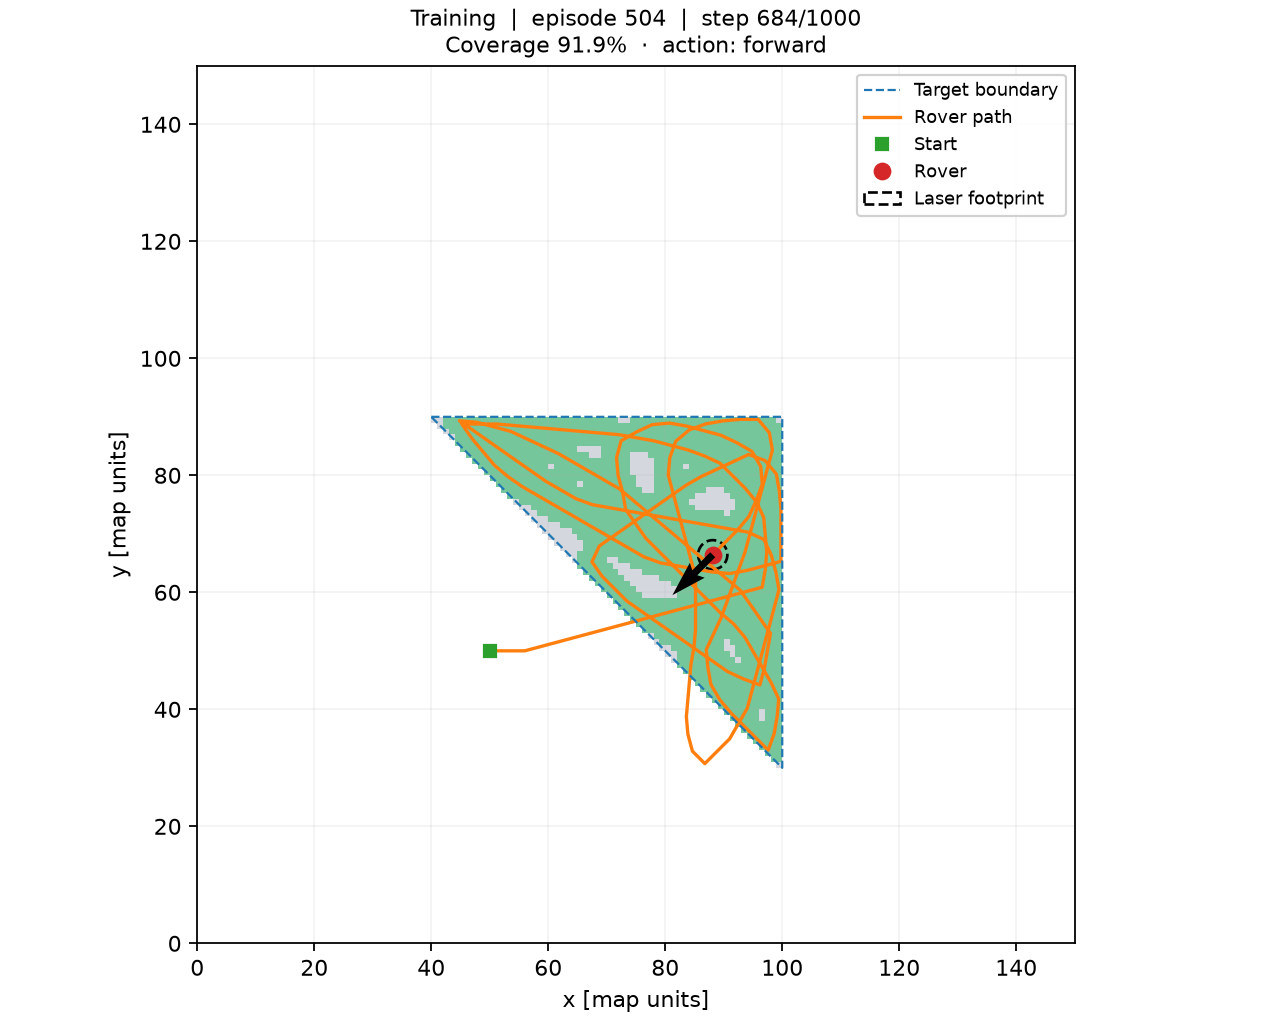
\includegraphics[width=0.3\textwidth, keepaspectratio]{./images/triangle_500episodes/rover.png}
  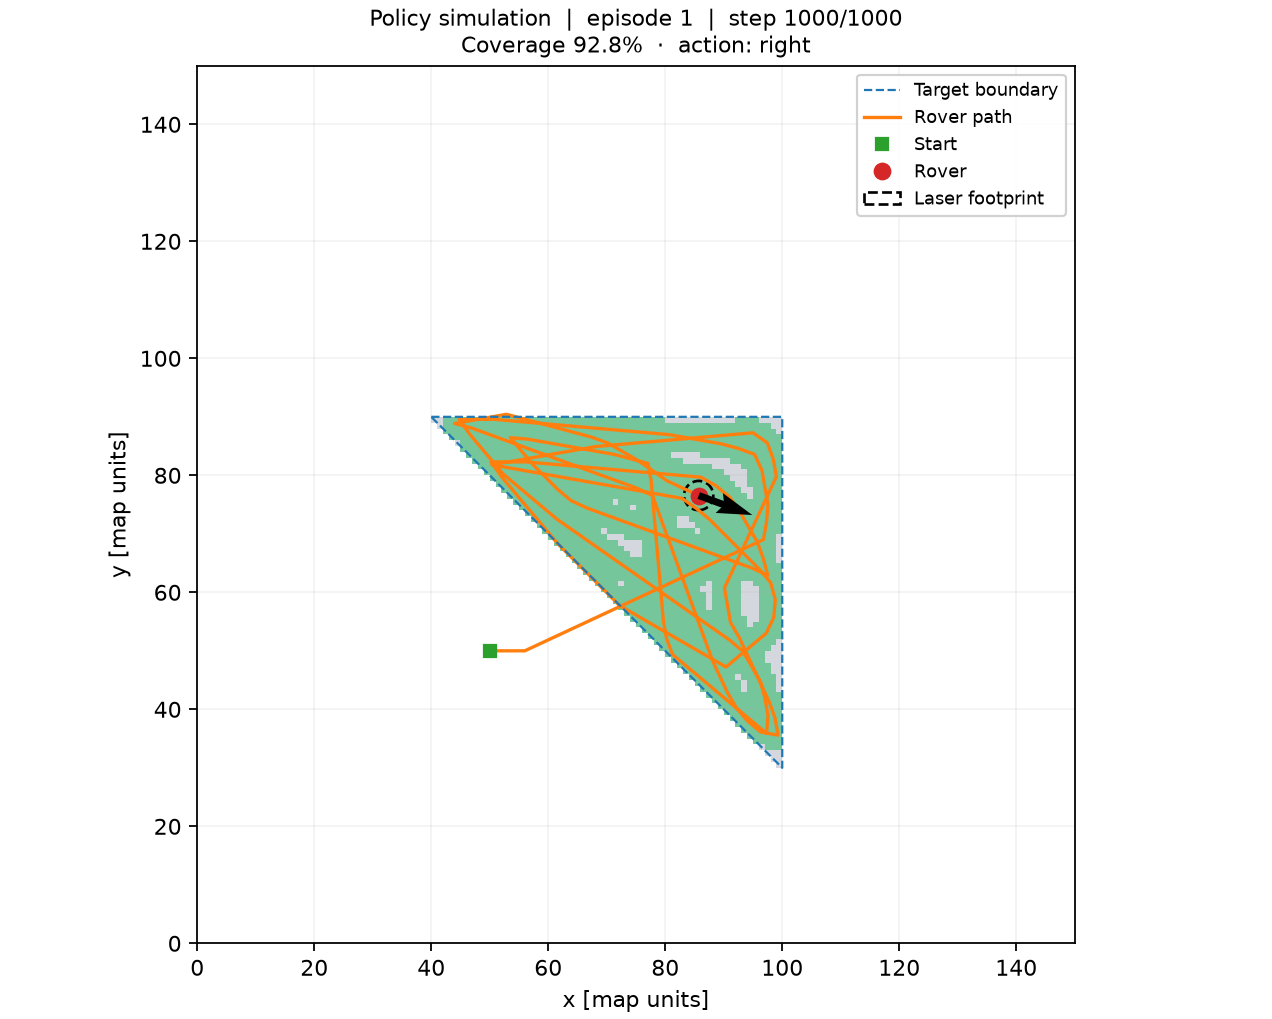
\includegraphics[width=0.3\textwidth, keepaspectratio]{./images/triangle_1000episodes/rover.png}
  \caption{Comparison of scanning trajectories after 250, 500 and 1000 training episodes\label{training_output_trian_fig}}
\end{figure}

\begin{figure}[H]
  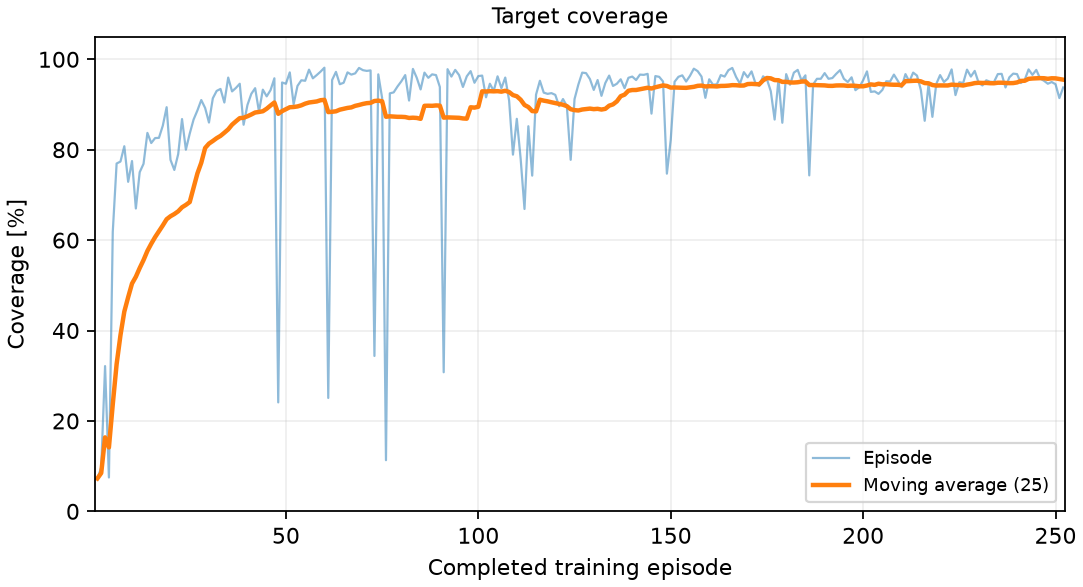
\includegraphics[width=0.3\textwidth, keepaspectratio]{./images/triangle_250episodes/coverage.png}
  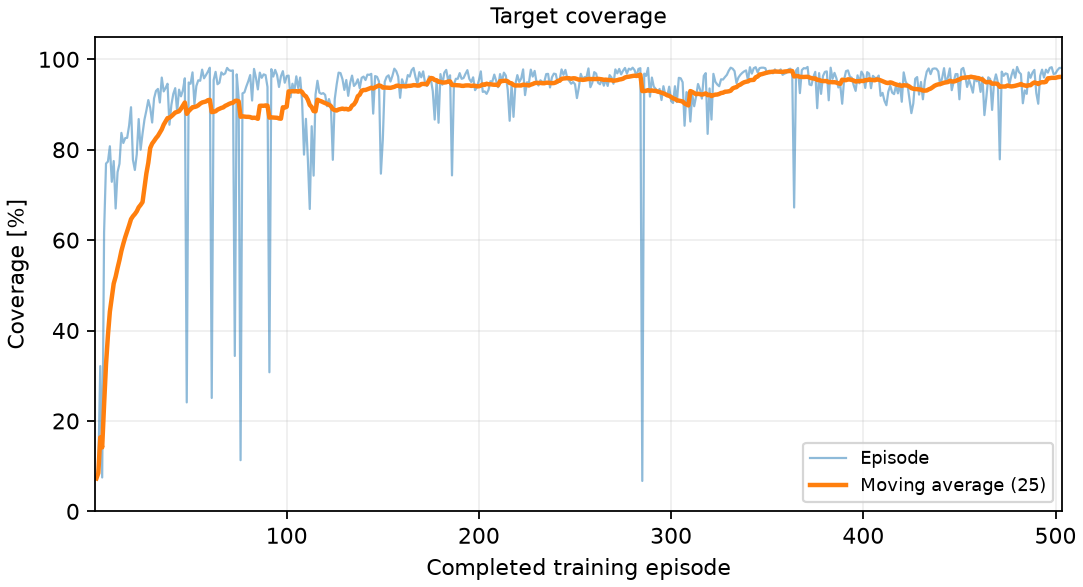
\includegraphics[width=0.3\textwidth, keepaspectratio]{./images/triangle_500episodes/coverage.png}
  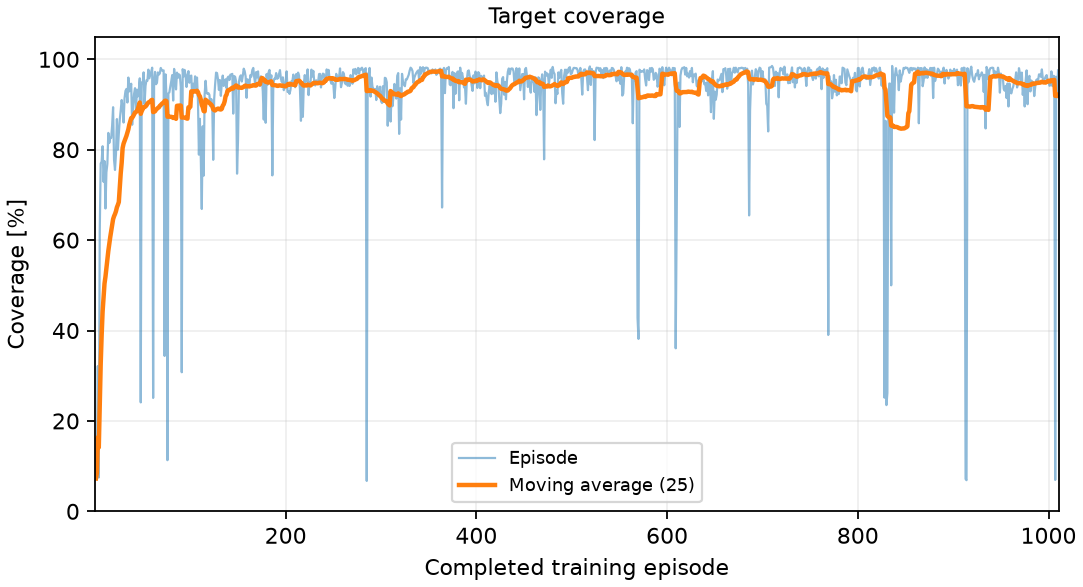
\includegraphics[width=0.3\textwidth, keepaspectratio]{./images/triangle_1000episodes/coverage.png}
  \caption{Surface coverage comparison\label{cover_trian_fig}}
\end{figure}

\begin{figure}[H]
  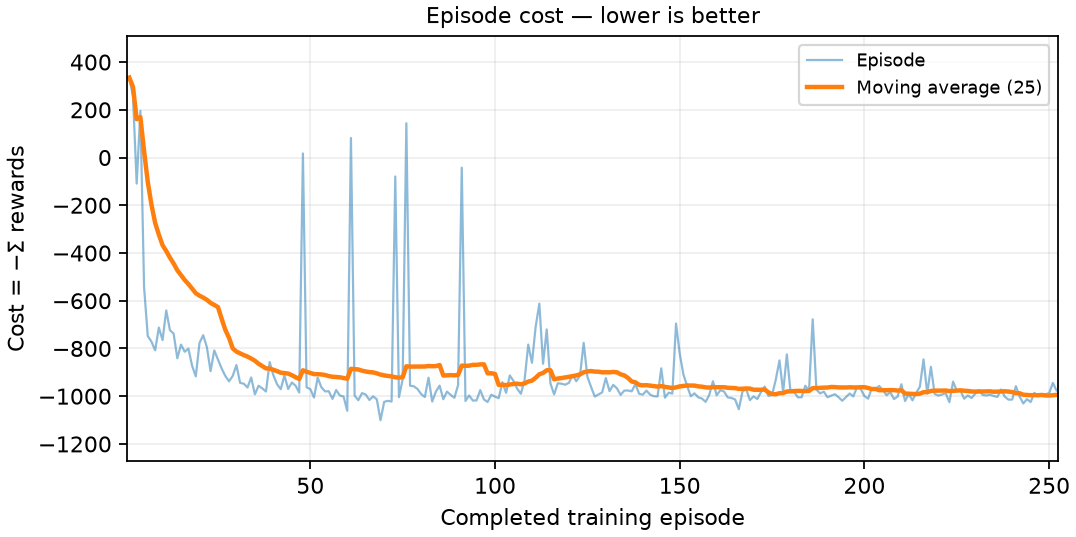
\includegraphics[width=0.3\textwidth, keepaspectratio]{./images/triangle_250episodes/episode_cost.png}
  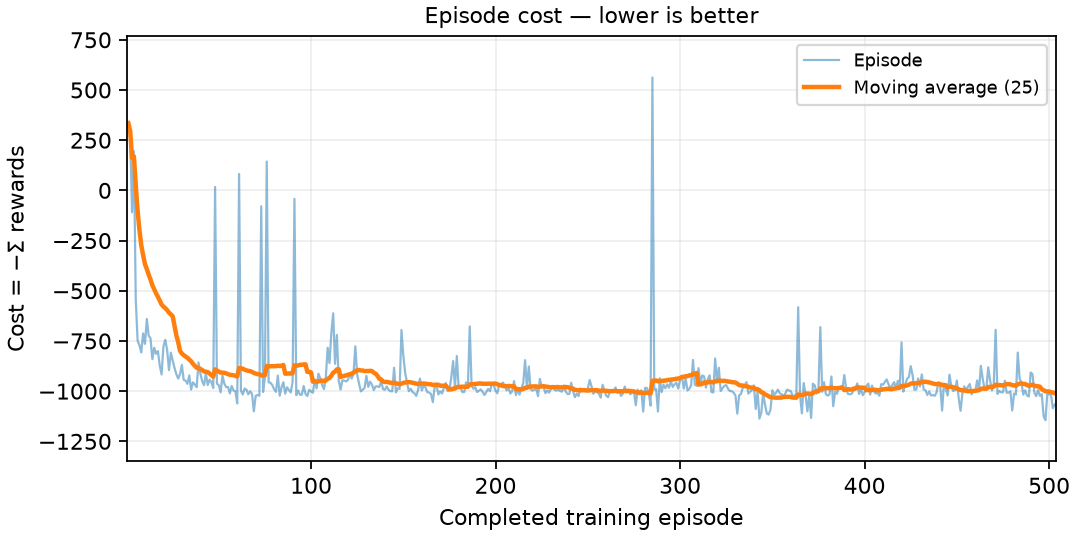
\includegraphics[width=0.3\textwidth, keepaspectratio]{./images/triangle_500episodes/episode_cost.png}
  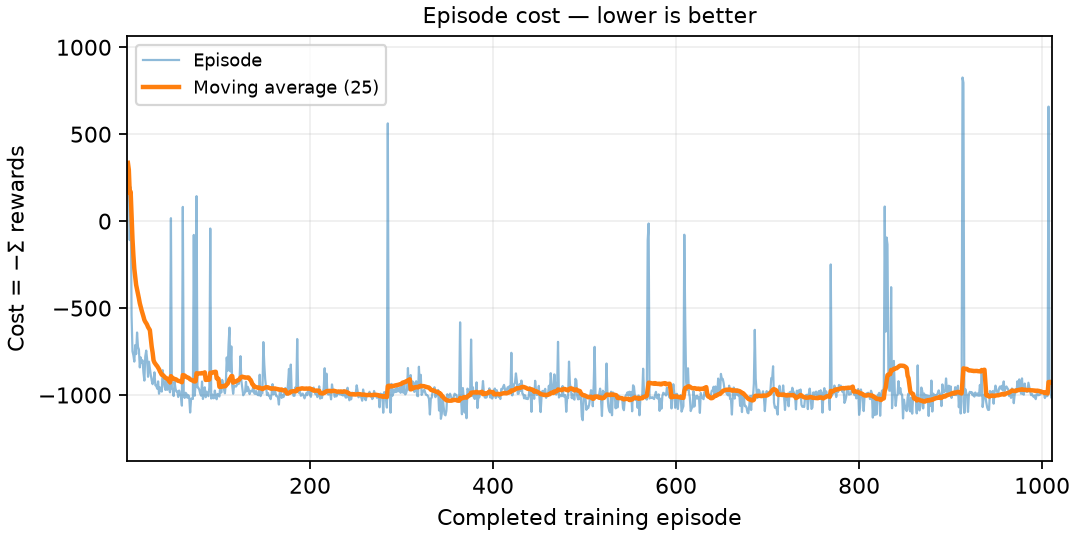
\includegraphics[width=0.3\textwidth, keepaspectratio]{./images/triangle_1000episodes/episode_cost.png}
  \caption{Cost comparison \label{cost_trian_fig}}
\end{figure}

\begin{figure}[H]
  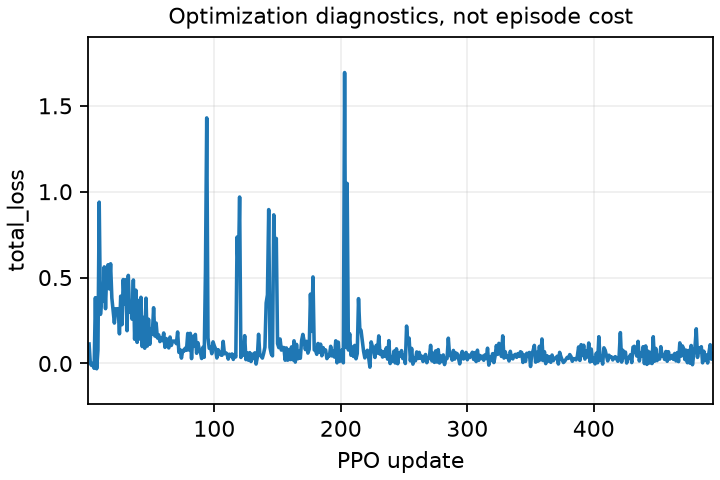
\includegraphics[width=0.3\textwidth, keepaspectratio]{./images/triangle_250episodes/ppo_loss.png}
  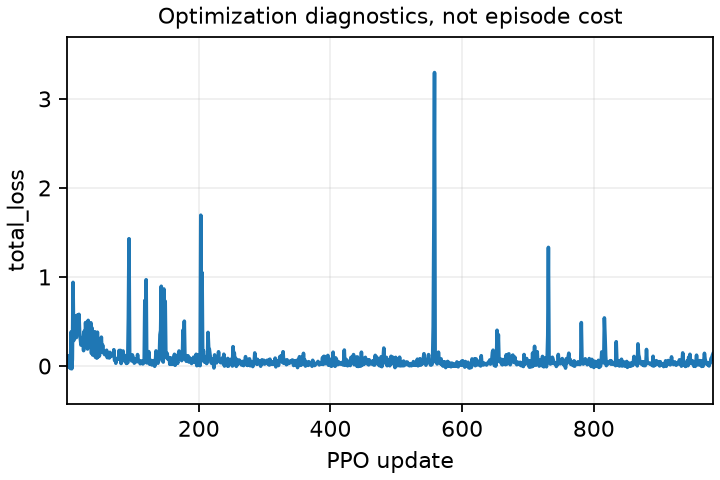
\includegraphics[width=0.3\textwidth, keepaspectratio]{./images/triangle_500episodes/ppo_loss.png}
  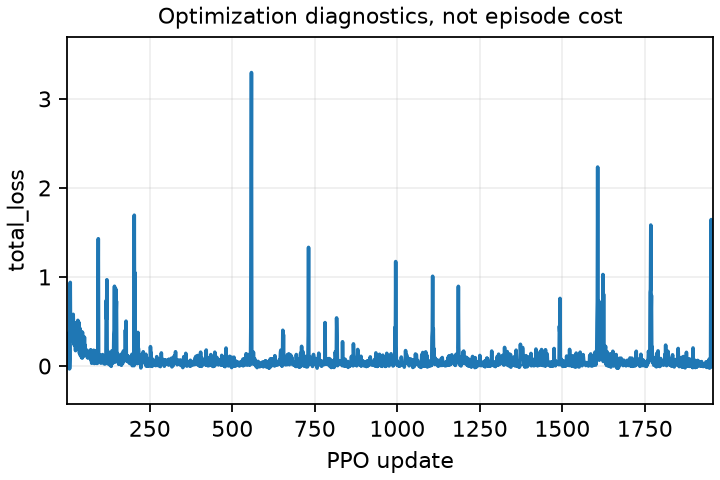
\includegraphics[width=0.3\textwidth, keepaspectratio]{./images/triangle_1000episodes/ppo_loss.png}
  \caption{Loss function comparison \label{loss_function_trian_fig}}
\end{figure}

Results of cost and loss functions for cicle \& triangle are similiar (figures \ref{cost_fig}, \ref{cost_trian_fig}, \ref{loss_function_fig} and \ref{loss_function_trian_fig}). As for the ellipse (figures \ref{cost_ellipse_fig} and \ref{loss_function_ellipse_fig}) the difference is observed mainly at the beginning of the training.

\begin{figure}[H]
  \centering
  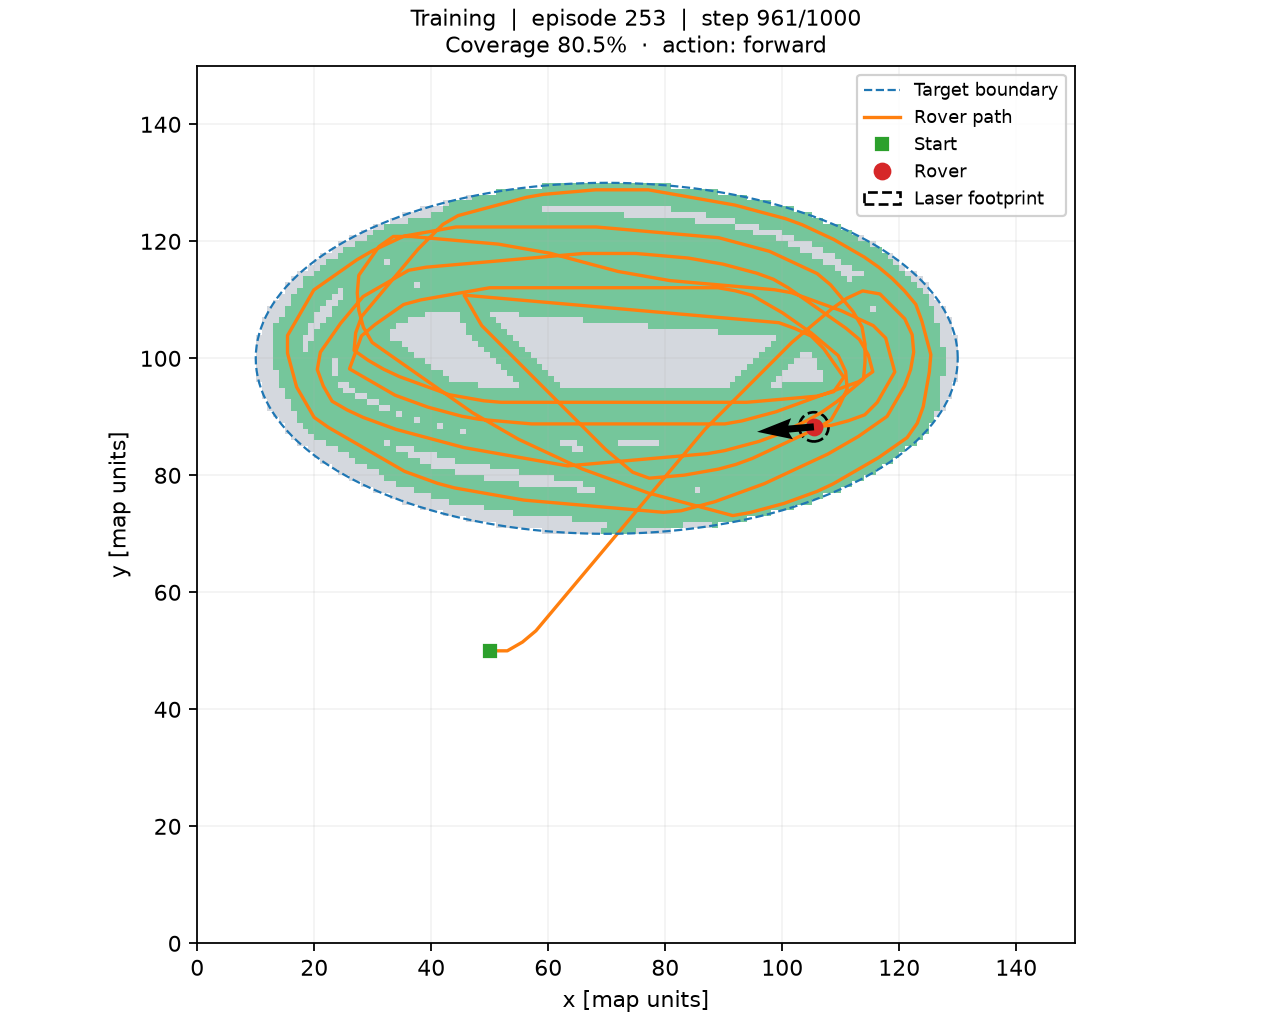
\includegraphics[width=0.3\textwidth, keepaspectratio]{./images/ellipse_250episodes/rover.png}
  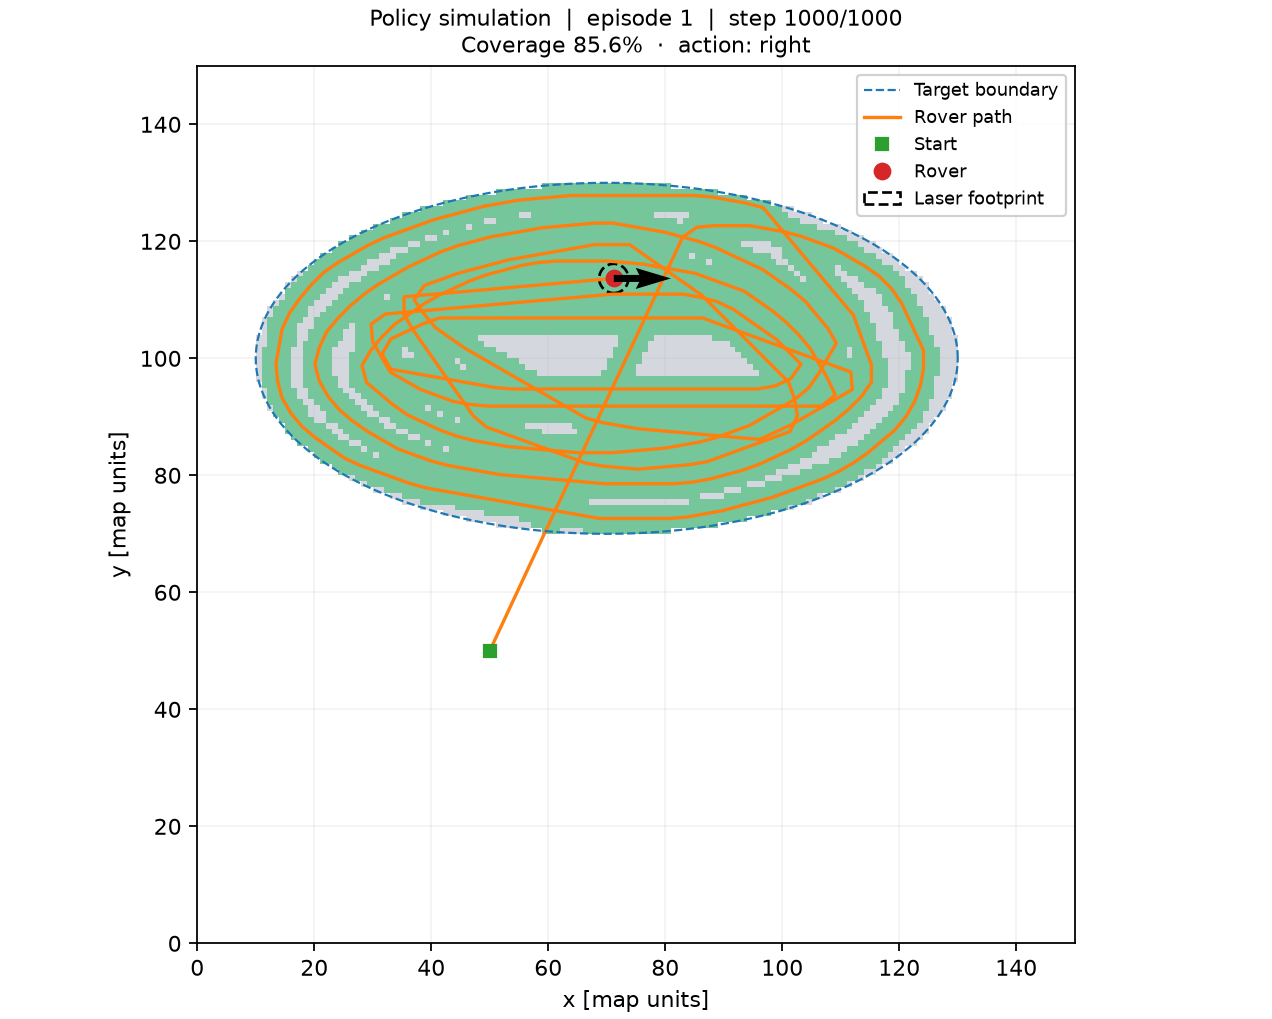
\includegraphics[width=0.3\textwidth, keepaspectratio]{./images/ellipse_500episodes/rover.png}
  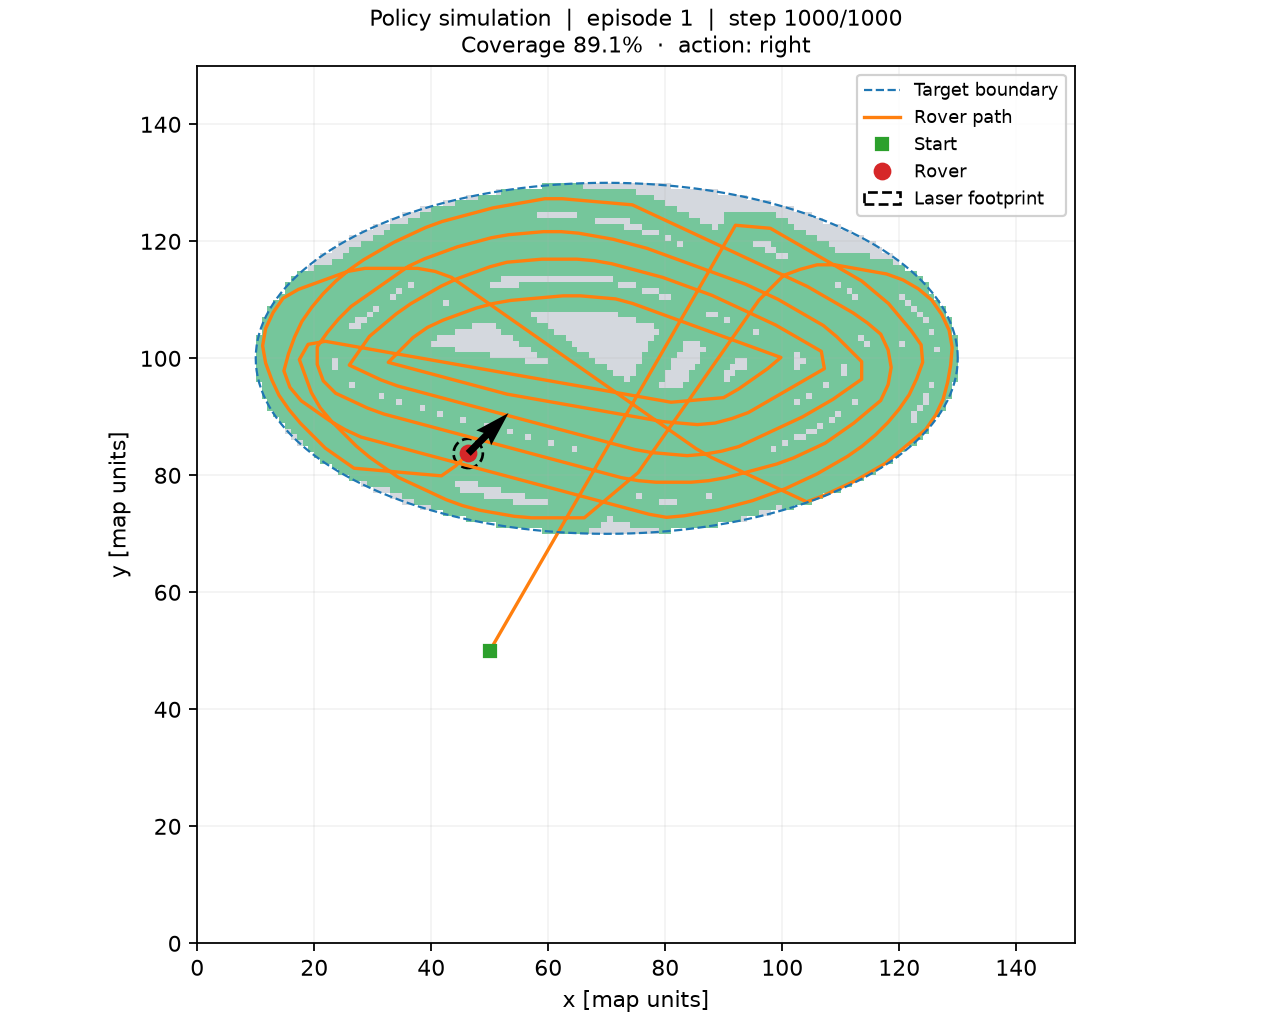
\includegraphics[width=0.3\textwidth, keepaspectratio]{./images/ellipse_1000episodes/rover.png}
  \caption{Comparison of scanning trajectories after 250, 500 and 1000 training episodes\label{training_output_ellipse_fig}}
\end{figure}

\begin{figure}[H]
  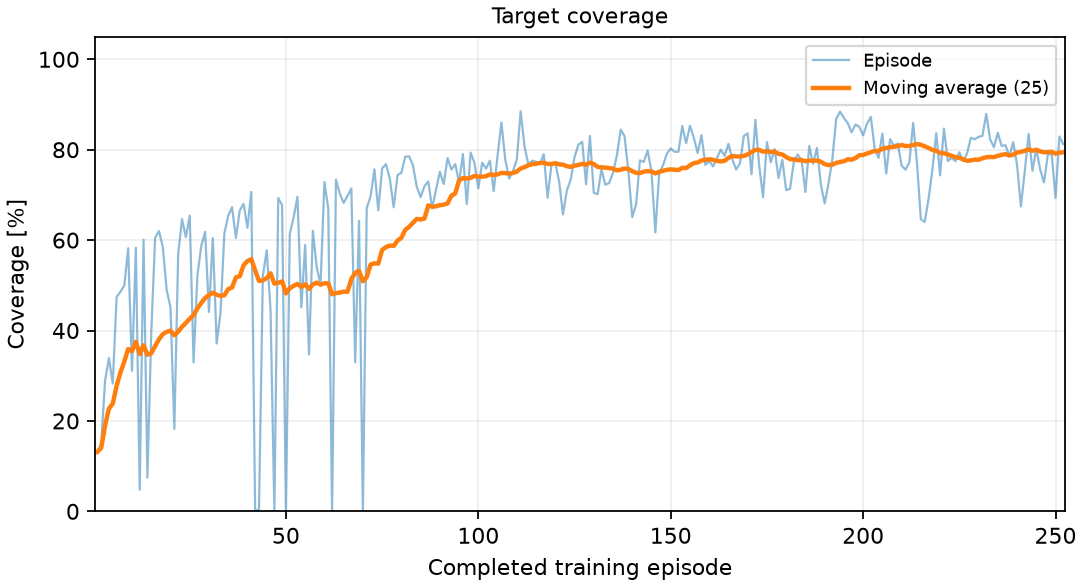
\includegraphics[width=0.3\textwidth, keepaspectratio]{./images/ellipse_250episodes/coverage.png}
  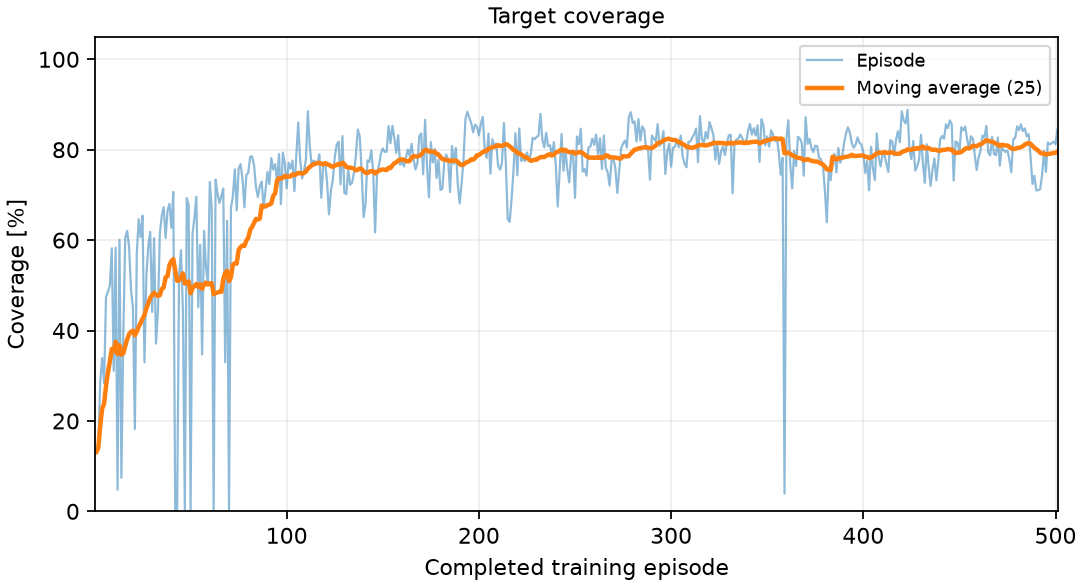
\includegraphics[width=0.3\textwidth, keepaspectratio]{./images/ellipse_500episodes/coverage.png}
  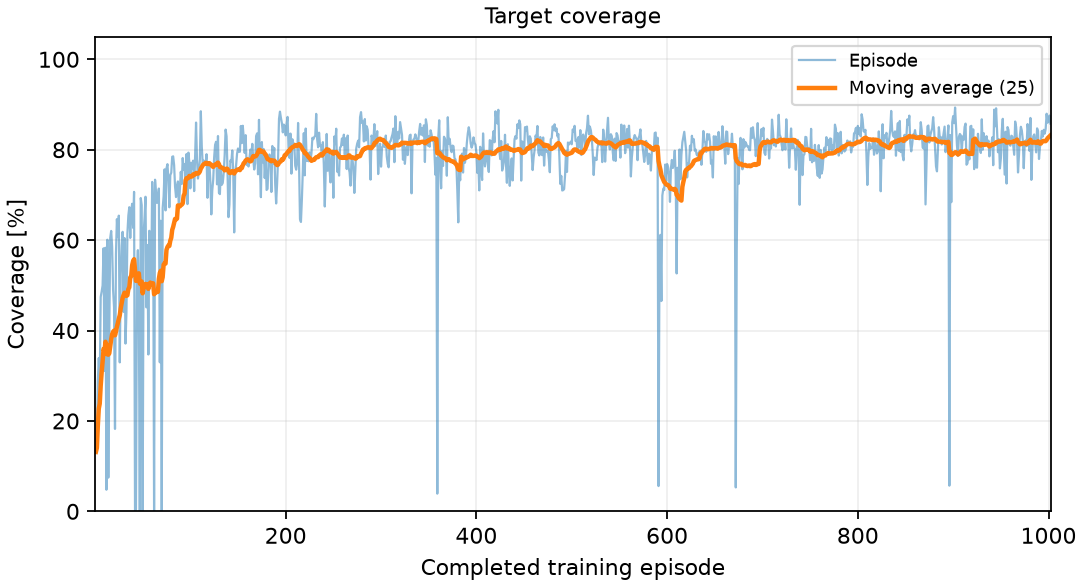
\includegraphics[width=0.3\textwidth, keepaspectratio]{./images/ellipse_1000episodes/coverage.png}
  \caption{Surface coverage comparison\label{cover_ellipse_fig}}
\end{figure}

\begin{figure}[H]
  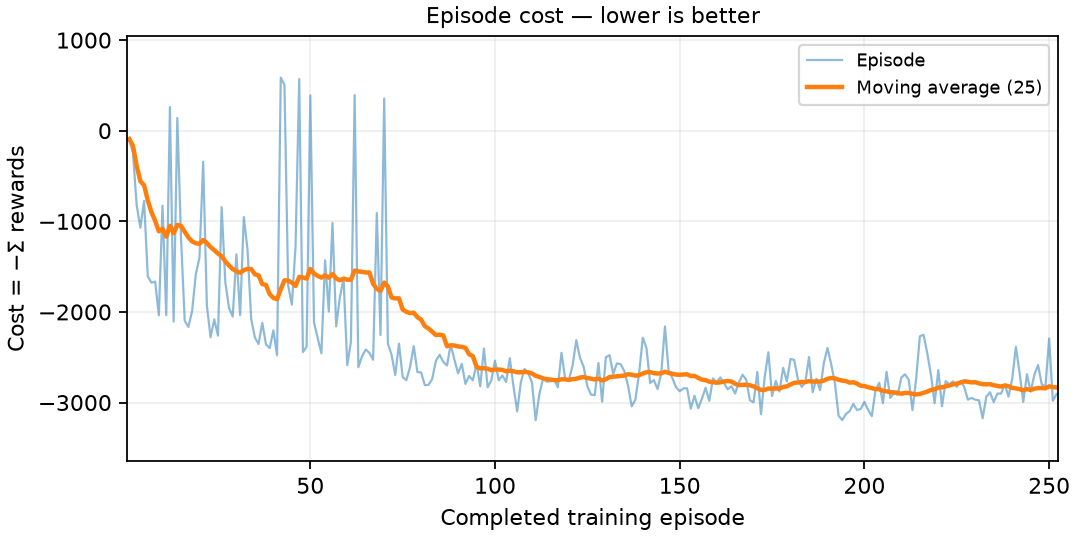
\includegraphics[width=0.3\textwidth, keepaspectratio]{./images/ellipse_250episodes/episode_cost.png}
  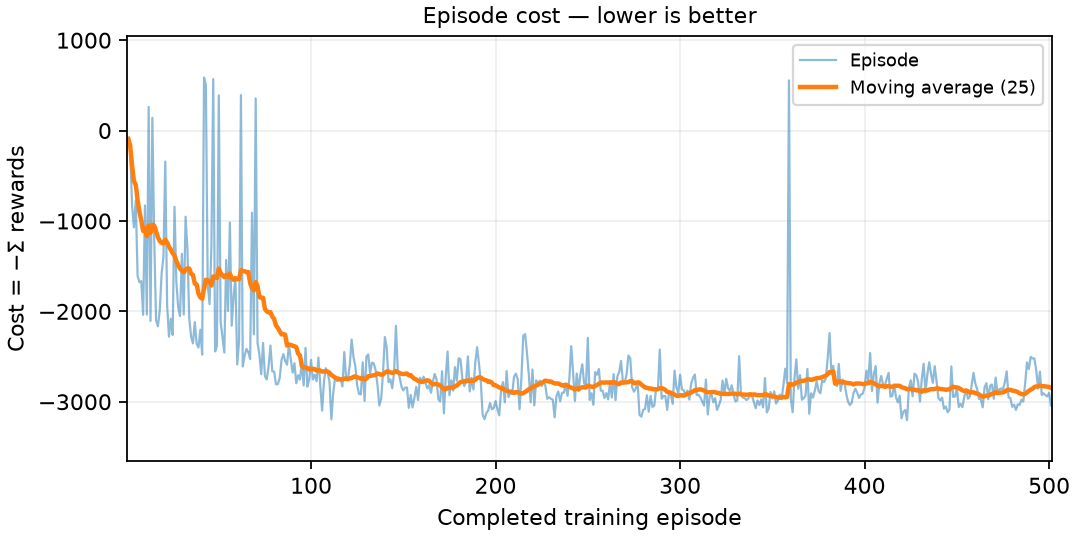
\includegraphics[width=0.3\textwidth, keepaspectratio]{./images/ellipse_500episodes/episode_cost.png}
  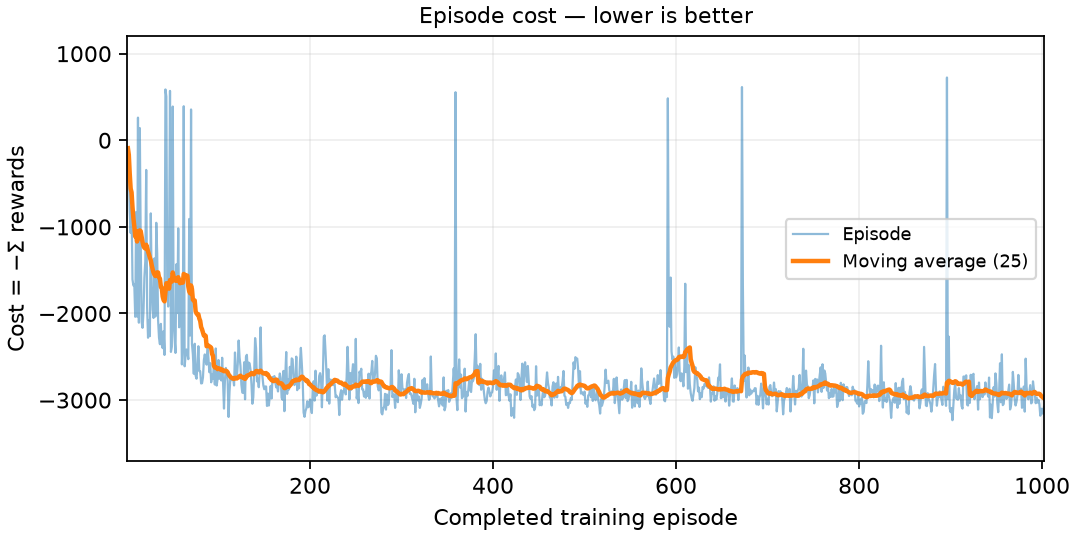
\includegraphics[width=0.3\textwidth, keepaspectratio]{./images/ellipse_1000episodes/episode_cost.png}
  \caption{Cost comparison \label{cost_ellipse_fig}}
\end{figure}

\begin{figure}[H]
  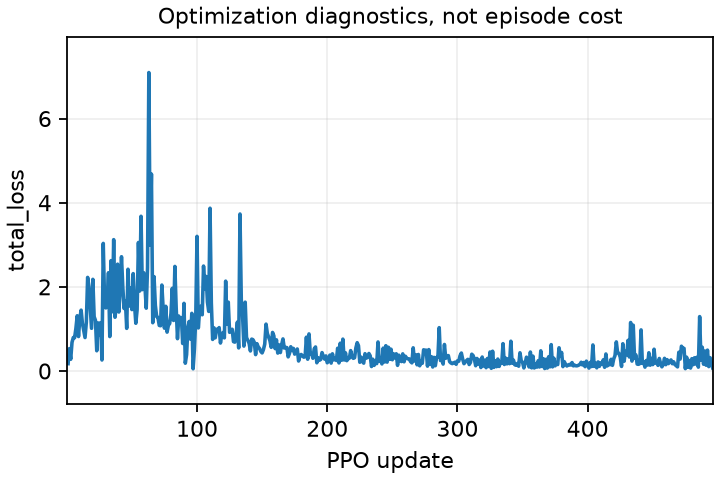
\includegraphics[width=0.3\textwidth, keepaspectratio]{./images/ellipse_250episodes/ppo_loss.png}
  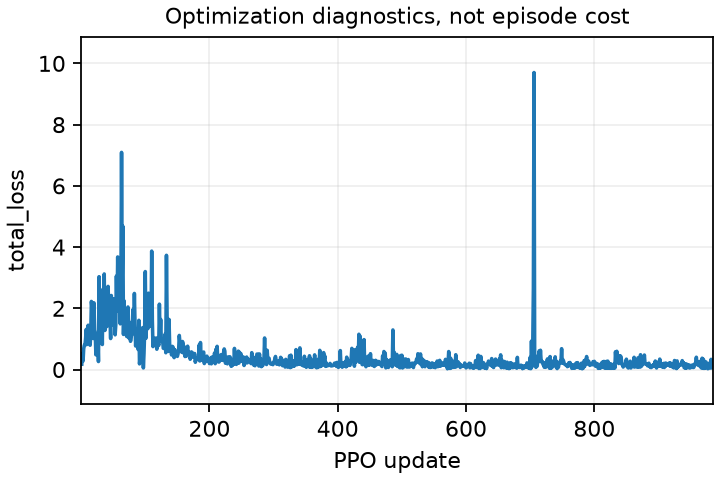
\includegraphics[width=0.3\textwidth, keepaspectratio]{./images/ellipse_500episodes/ppo_loss.png}
  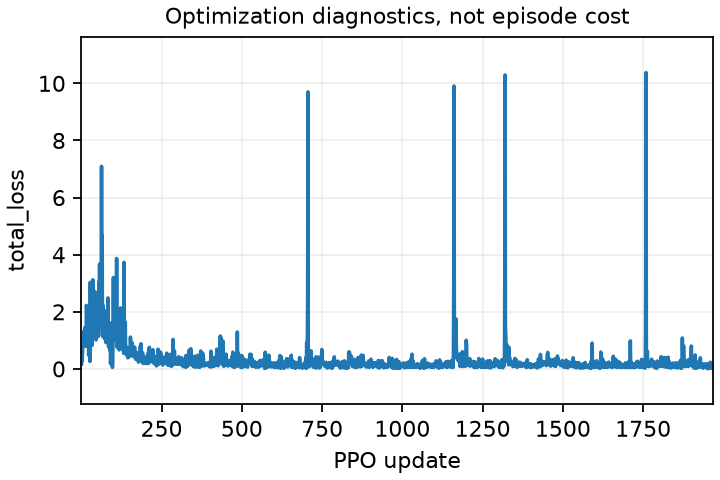
\includegraphics[width=0.3\textwidth, keepaspectratio]{./images/ellipse_1000episodes/ppo_loss.png}
  \caption{Loss function comparison \label{loss_function_ellipse_fig}}
\end{figure}

\section{Results \& Discussion}
The comparison of different training stages highlights several important aspects of PPO-based coverage planning. Increasing the number of training episodes does not necessarily improve scanning performance, as suggested by the behavior observed after 1000 episodes. Furthermore, achieving high surface coverage does not guarantee an efficient trajectory, since previously scanned areas may be revisited. These observations emphasize the importance of balancing coverage, path efficiency, and training stability. Further evaluation is required to determine whether the observed performance differences result from the reward function, policy updates, or variations between training runs (different seeds). Important notice for choosing a seed, sometimes agent is stuck in minigless constant rotations. It is coused by reward system, the agent treat rotating as lesser punishment than exploring on its own. The unexpected begin could be coused by random movement to find the object like in ellipse example. The rover must explore the envinronment before it starts to scan.

\section{Conclusion}

The presented results don't prove that classical mathematical approaches are inferior to Machine Learning techniques. A trained AI agent can compete with analytical geometric decomposition because of its potential ability to adapt its policy to new aircraft geometries that were not included in training guarantee model self-adjustment. Changing aircraft geometries requires decomposing new plane geometries into simpler shapes using geometry decomposition instead of using an AI model. Simple shapes such as rectangles, circles, triangles can be used to train specialized models. Overfitting may occur after 1000 episodes. However, it is also possible that the simulation is unstable and overfitting is not occurring (it is too early to draw a definitive conclusion). The model could be trained on one shape and used by a higher level agent supervising its operations. This way the model could improve the probability of successful scanning without losing idea of circular shape by retraining for second or third shape recognition. In aircraft maintenance this solution could evolve into an autonomous system. In the final project communication with the rover(s) will be established via WebSocket connections to enable bidirectional communication and better solution in comparison with conventional HTTP requests \cite{kufa2025pathplanning}. This communication channel is established between the server and the clients as well as between the server and the container (database).


\bibliographystyle{unsrtnat}
\bibliography{references}

\end{document}

